\documentclass{article}


\usepackage{newspaper}
\date{September 14, 2013}
\currentvolume{1}
\currentissue{1}
\usepackage[utf8]{inputenc}
\usepackage{times}
\usepackage{graphicx}
\usepackage{multicol}
\usepackage{verse}
\usepackage[small,unboxed]{cwpuzzle}
\usepackage[nonumber]{cuisine}
%\RecipeWidths{\textwidth}{.20cm}{3cm}{2.50cm}{.85cm}{1.85cm}

\usepackage{picinpar}
%uasage of picinpar:
%\begin{window}[1,l,\includegraphics{},caption]xxxxx\end{window}

%%%%%%%%%  Front matter   %%%%%%%%%%

\SetPaperName{Jorels:ea Journal}
\SetHeaderName{Jorelsea Journal}
\SetPaperLocation{San Francisco}
\SetPaperSlogan{Our paper's slogan!}
\currentvolume{1}
\currentissue{1}
\SetPaperPrice{75 CENTS}

\begin{document}
\maketitle

\begin{multicols}{3}
    \byline{\Large Commuter Marvel}{Lisa Eldredge}
    The route to preschool was walkable but the school was situated near the
    top of a very steep hill. At the time Jordan loved to roller skate. One
    morning instead of walking to school he wanted to skate. I agreed, thinking
    that he would soon find the hill too steep and we'd be carrying the skates.
    We set off down our hill then up the slope to the school. Cheerfully making
    slow and steady progress he made it to the top. Along the way his
    classmates passed us by in their cars and cheered him on.

    Jordan made the commute to school by roller skate most of the rest of the
    year, garnering plenty of awe and admiration for his patience and prowess
    to conquer that hill every morning.
    \closearticle

    \byline{\Large Boy Defies Mother}{Lisa Eldredge}
    Before Kindergarten school-picture day Jordan came home very excited
    proposing that he wear our dress-up band jacket and hat. I agreed but on
    the condition that he take off the hat for the photo and hold it in his
    lap. He wasn't too happy with that idea but agreed. A few weeks later when
    the photos came, there looking at me from the glossy photo was the happiest
    5 year old you have ever seen. Upright and glowing in the red band jacket
    and most notably, the white patent leather hat perched proudly on his head.
    I smiled back at the image, hugged Jordan for such a wonderful photo,
    noting that my heart was so glad for his joy that I had no motivation to
    reprimand him.

    Moral of the story: Play it safe. If you are going to defy your mother,
    don't have someone take a photo of you in the act.
    %\closearticle
 
    \columnbreak
    \byline{\Large Reading}{Alexandrea Kelly}
    \byline{\Large Reading}{Alexandrea Kelly}
\settowidth{\versewidth}{was the scent of French fries}
\begin{verse}[\versewidth]
On my favorite vacation\\
in the state of 10,000 lakes\\
We went on a boat ride\\
one was especially great\\
\end{verse}

\begin{verse}[\versewidth]
On our way back\\
we had to make a stop\\
We went turtle hunting\\
on a restaurant dock\\
\end{verse}

\begin{verse}[\versewidth]
All that I could smell\\
was the scent of French Fries\\
All that I could hear\\
was the laughter + cries\\
\end{verse}

\begin{verse}[\versewidth]
We looked in the water\\
with not much luck\\
Searching for turtles\\
all we could see was muck\\
\end{verse}

\begin{verse}[\versewidth]
While looking off\\
one of the sides\\
I saw my friend Chelsea\\
in the corner of my eye\\
\end{verse}

\begin{verse}[\versewidth]
I just couldn't help\\
but push her in\\
Afterward I would regret\\
what I had did\\
\end{verse}

\begin{verse}[\versewidth]
I ran to the boat\\
and wouldn't get out\\
Then all I heard were\\
screams + shouts\\
\end{verse}

\begin{verse}[\versewidth]
When we finally got home\\
what I deserved I got\\
Five pushes in the lake\\
that was sure alot\\
\end{verse}



    \columnbreak
    \byline{\Large Jumble}{Lisa Eldredge}
    Unscramble these six Jumbles, one letter to each square, to form six words.\\

\begin{Puzzle}{10}{2}
|[][SLTB]E|[][STB]K|[][STB]L|[][STB]U|[][STB]L|[][STB]U|[][SRTB]E|[][.]X|[][.]X|[][.]X|.
|[][.]X|[][.]X|[][.]X|[][o]U|K|[][o]U|L|[][o]E|L|E|.
\end{Puzzle}
Hint: Jordan serenades Chelsea with this.\bigskip

\begin{Puzzle}{10}{2}
|[][SLTB]T|[][STB]R|[][STB]I|[][STB]B|[][STB]E|[][STB]A|[][STB]N|[][SRTB]O|[][.]X|[][.]X|.
|[][.]X|[][.]X|[][o]T|R|I|[][o]B|E|A|N|O|.
\end{Puzzle}
Hint: Jordan serenades Chelsea with this too!\bigskip

\begin{Puzzle}{10}{2}
|[][SLTB]A|[][STB]R|[][STB]O|[][STB]O|[][STB]T|[][STB]A|[][STB]C|[][STB]L|[][STB]U|[][SRTB]R|.
|[][o]A|R|O|O|T|A|[][o]C|[][o]L|U|R|.
\end{Puzzle}
Hint: Chelsea is amazing!\bigskip

\begin{Puzzle}{10}{2}
|[][SLTB]P|[][STB]O|[][STB]L|[][STB]Y|[][STB]I|[][STB]A|[][SRTB]M|[][.]X|[][.]X|[][.]X|.
|[][.]X|[][.]X|[][.]X|P|O|L|[][o]Y|I|[][o]A|M|.
\end{Puzzle}
Hint: She's a doll.\bigskip

\begin{Puzzle}{10}{2}
|[][SLTB]P|[][STB]E|[][STB]O|[][STB]N|[][STB]A|[][STB]G|[][STB]P|[][SRTB]A|[][.]X|[][.]X|.
|[][.]X|[][.]X|P|[][o]A|P|A|G|E|N|O|.
\end{Puzzle}
Hint: He's a birdman.\bigskip

\begin{Puzzle}{10}{2}
|[][SLTB]F|[][SRTB]S|[][.]X|.
|[][.]X|[][o]F|[][o]S|.
\end{Puzzle}
Hint: The city where this true love began and flourishes!\bigskip

Now arrange the circled letters to solve the equation:\bigskip

{\bf Jordan + Chelsea =}\bigskip

\begin{Puzzle}{10}{1}
|[][o]X|[][o]X|[][o]X|[][o]X|[][o]X|[][o]X|[][o]X|[][o]X|[][o]X|.
\end{Puzzle}

\begin{Puzzle}{10}{1}
|[][o]X|[][o]X|[][o]X|[][o]X|[][o]X|.
\end{Puzzle}


\end{multicols}
\pagebreak

\begin{multicols}{2}
    \columnbreak
    \byline{\Large Tea Leaves}{Patty Hollow}
    \byline{\Large Tea Leaves}{Patty Hollow}
I thought this old poem I wrote was apropos of my grandmother's old tea cups, which I gave Chelsea and Jordan.

\bigskip
{\centering
    You hold me like an antique sugar spoon,\\
    delicate with rounded valley's, curved\\
    to catch the sweentess of my bite.\\
    The intricate Olde English filigree handle\\
    you caress exposes my secret crevasses\\
    polished now to a fine rich patina.\\
    I become as warm and liqud as the amber\\
    Oolong leaves sweetened by rainbow crystals\\
    poured from my gradmother's hand\\
    rubbed silver tea pot.\\
}

    \byline{\Large Photographs}{Andrée Young}
    \byline{\Large Photographs}{Andrée Young}
\begin{window}[0,c,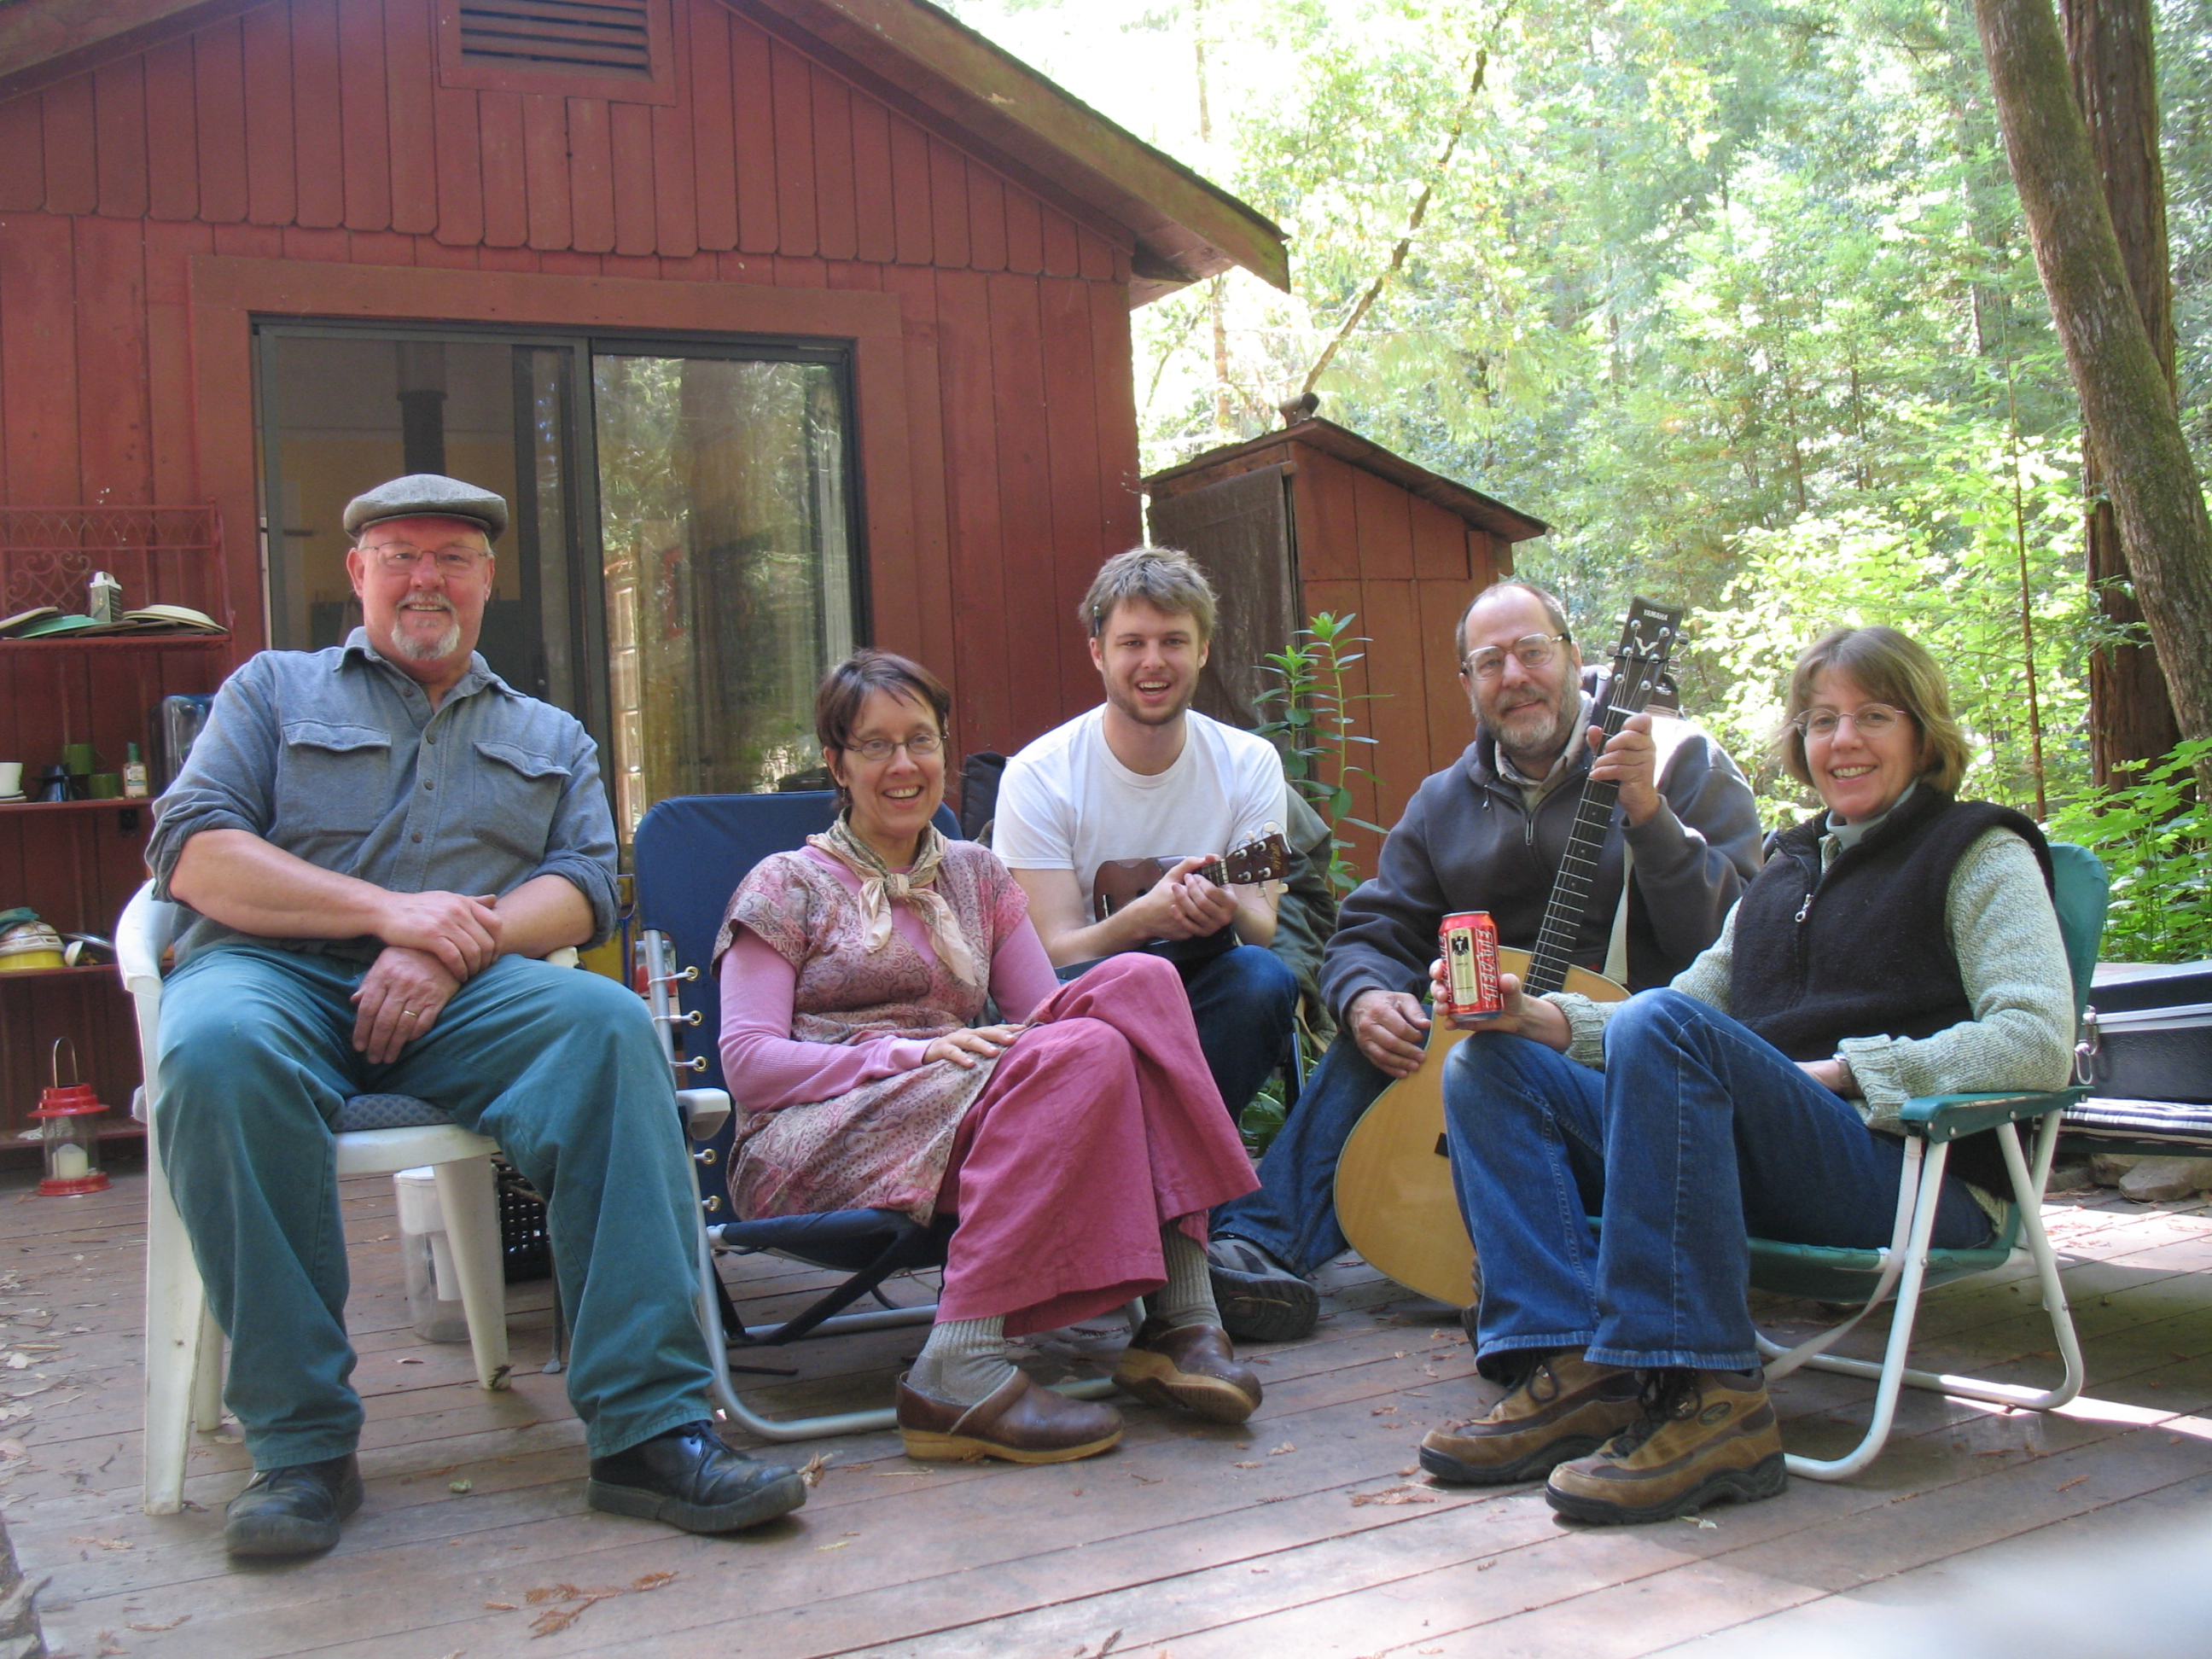
\includegraphics[width=3.4in]{includes/reeves_canyon.jpg},{\centering David, Lisa, Jordan, Gilbert and Andrée}]
\smallskip
This photo of Jordan at The Forest of Dreams is from Sept. 7, 2009. It was
a year after our son, David's death and I was still recovering from
a Bilateral Mastectomy on July 22, 2009. Lisa and Gilbert invited David and
I to stay with them. I remember Jordan's kindness and walking to the top of
a little hill nearby with Jordan by my side. Of course there was music and
a dirty word scrabble game in which Jordan was my partner.
\end{window}

\begin{window}[0,c,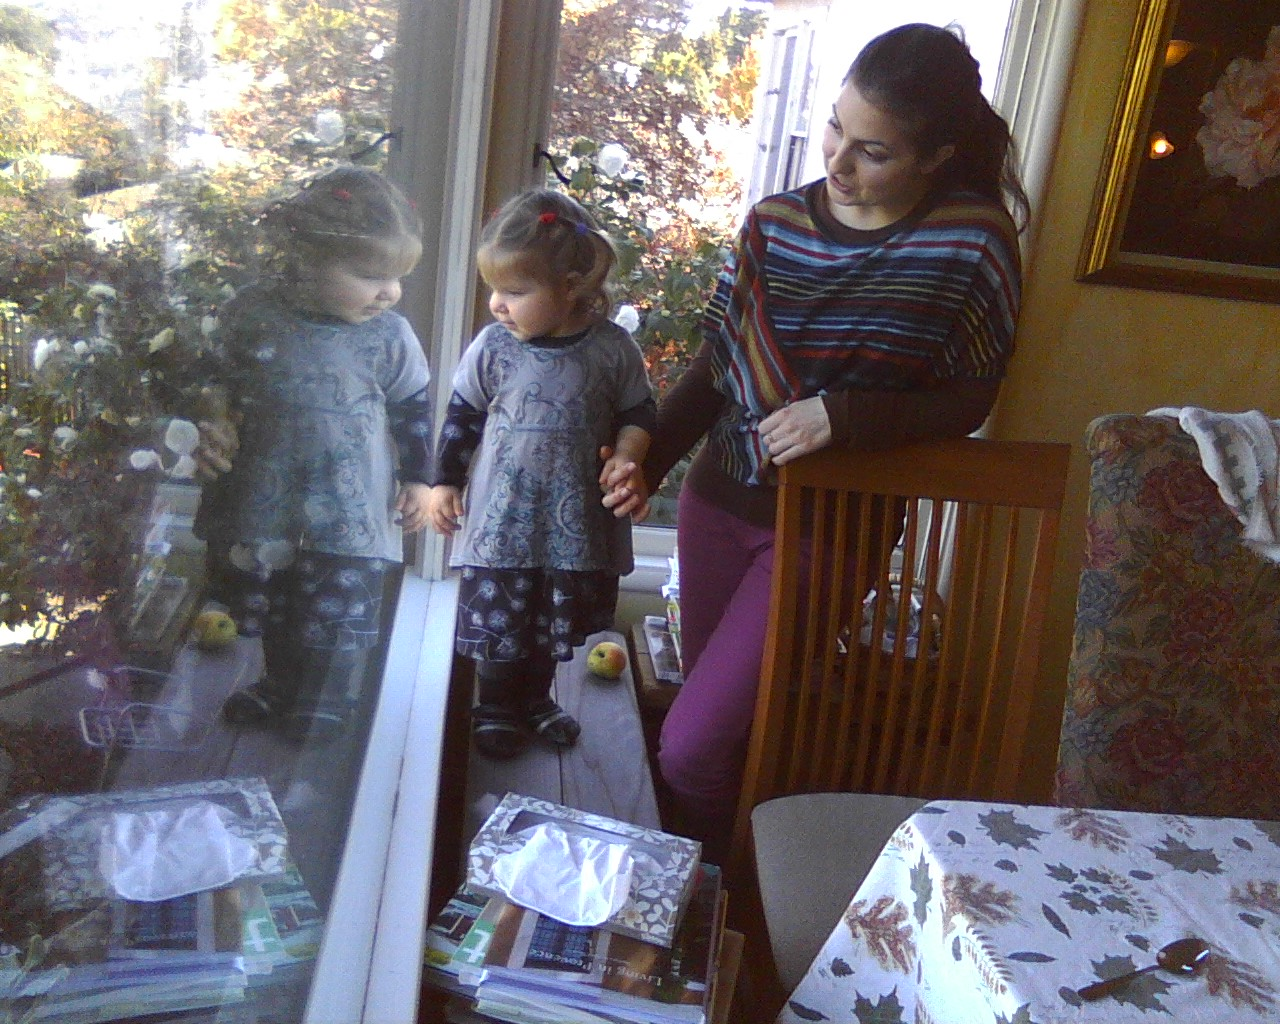
\includegraphics[width=3.4in]{includes/chelsea_and_aviva.jpg},{\centering Aviva and Chelsea}]
\smallskip
This photo of Chelsea and Aviva is from New Year's Eve, 2012, shortly after or
before she entertained us with the mechanical doll aria from {\it Tales of
Hoffmann}. Aviva said, ``Again!'' and she did it again.
\end{window}



    \byline{\Large Die Rose, die Lilie}{Jordan Eldredge} I first learned this
    Heinrich Heine poem as part of Robert Schumann's {\it Dichterliebe} song
    cycle. This cycle has always been special to me. One of the first birthday
    gifts I gave to Chelsea was wrapped in it's sheet music. The first piece of
    jewelry I gave to Chelsea was a silver ring in a decorated matchbox
    inscribed with this poem.

    Recently I asked Chelsea to choose the inscription for the inside of my
    wedding band. She chose ``Die Eine''.

    \settowidth{\versewidth}{the little one, the dainty one, the pure one, the One.}
    \begin{verse}[\versewidth]
    Die Rose, die Lilie, die Taube, die Sonne,\\
    Die liebt' ich einst alle in Liebeswonne,\\
    Ich lieb' sie nicht mehr, ich liebe alleine\\
    Die Kleine, die Feine, die Reine, die Eine;\\
    Sie selber, aller Liebe Wonne,\\
    Ist Rose und Lilie und Taube und Sonne.\\
    \end{verse}
    \settowidth{\versewidth}{the little one, the dainty one, the pure one, the One.}
    \begin{verse}[\versewidth]
    The rose, the lily, the dove, the sun-\\
    I once loved them all with ecstatic love.\\
    I love them no more, I love only\\
    the little one, the dainty one, the pure one, the One.\\
    She alone, the well-spring of all love,\\
    is rose and lily and dove and sun.\\
    \end{verse}

    \columnbreak
    \pagebreak
    \headline{\Large Birth Announcement}
    \headline{\Large Birth Announcement}
Baby boy, Jordan Daniel Bartsch Eldredge born March 11, 1985, 5:43am, 7lbs 6oz
to Lisa and Gilbert Eldredge at home in Petaluma California.  Present at the
birth were his Papa, Gilbert, and brother, Nathaniel.  Toast with loads of
butter was served by dear friend Nora immediately following.  Special note that
the 10\textsuperscript{th} of March was an auspicious day with rainbows
throughout.


    \closearticle
    % Crossword puzzle
    \byline{\Large Crossword}{Chelsea Hollow \& Jordan Eldredge}
    \begin{Puzzle}{14}{20}
|*    |[1]Z |[2]I |[3]G |Z    |[4]A |[5]G |*    |*    |[6]H |[7]I |[8]P |*    |*    |.
|[9]T |I    |E    |R    |*    |[10]N|A    |[11]T|[12]H|A    |N    |I    |[13]E|[14]L|.
|[15]A|T    |*    |[16]A|[17]M|*    |[18]S|O    |A    |P    |*    |*    |[19]M|I    |.
|[20]T|H    |O    |M    |A    |S    |*    |[21]S|I    |P    |*    |[22]P|U    |N    |.
|[23]T|E    |*    |[24]P|S    |*    |[25]T|H    |R    |I    |[26]C|E    |*    |E    |.
|[27]O|R    |[28]C|A    |S    |[29]H|*    |*    |*    |[30]N|O    |D    |[31]E|S    |.
|O    |*    |I    |*    |*    |[32]O|[33]L|I    |[34]V|E    |O    |I    |L    |*    |.
|*    |[35]C|A    |[36]S|[37]T|R    |O    |*    |[38]E|S    |M    |A    |S    |*    |.
|[39]F|A    |*    |[40]C|O    |N    |V    |E    |R    |S    |E    |*    |[41]E|[42]D|.
|*    |[43]S|W    |I    |M    |*    |E    |*    |S    |*    |[44]O|J    |*    |O    |.
|*    |T    |*    |E    |*    |*    |R    |*    |[45]E|[46]L|F    |*    |[47]T|N    |.
|*    |*    |*    |[48]N|[49]E|W    |*    |*    |[50]S|O    |F    |[51]T|I    |E    |.
|[52]G|[53]R|A    |C    |E    |*    |[54]C|*    |*    |B    |*    |[55]R|E    |I    |.
|[56]R|E    |*    |[57]E|L    |[58]B|O    |[59]W|*    |[60]S|[61]T|Y    |*    |N    |.
|[62]O|L    |[63]E|*    |*    |[64]R|O    |E    |*    |[65]T|I    |A    |[66]R|A    |.
|[67]O|I    |S    |E    |[68]A|U    |*    |*    |[69]J|E    |N    |N    |A    |*    |.
|[70]M|S    |T    |*    |[71]G|I    |[72]L|B    |E    |R    |T    |*    |[73]I|[74]M|.
|*    |H    |*    |[75]M|A    |N    |I    |*    |L    |*    |*    |[76]O|N    |E    |.
|*    |*    |[77]B|L    |I    |S    |S    |*    |[78]L|[79]A|[80]U|D    |*    |M    |.
|[81]O|C    |E    |A    |N    |*    |[82]A|N    |Y    |W    |H    |E    |R    |E    |.
\end{Puzzle}


    \columnbreak
    \begin{multicols}{2}
        \begin{PuzzleClues}{\textbf{Across}}\\
\Clue{1}{ZIGZAG}{Switchback}\\
\Clue{6}{HIP}{Word with hop or joint}\\
\Clue{9}{TIER}{Wedding cake feature}\\
\Clue{10}{NATHANIEL}{Brother of 52 down}\\
\Clue{15}{AT}{@}\\
\Clue{16}{AM}{PM predecessor}\\
\Clue{18}{SOAP}{Bubble ingredient}\\
\Clue{19}{MI}{Third degree note}\\
\Clue{20}{THOMAS}{New brother to 52 down and 10 across}\\
\Clue{21}{SIP}{Tea quantity}\\
\Clue{22}{PUN}{Sichra groaner}\\
\Clue{23}{TE}{Tellurium symbol}\\
\Clue{24}{PS}{Letter afterthought}\\
\Clue{25}{THRICE}{Once and twice}\\
\Clue{27}{ORCASH}{``Credit \underline{\hspace{.75cm}}?''}\\
\Clue{30}{NODES}{Singer's afflictions}\\
\Clue{32}{OLIVEOIL}{Garlic and onion melder}\\
\Clue{35}{CASTRO}{Newlywed's neighborhood}\\
\Clue{38}{ESMAS}{``It is more'', South of the boarder}\\
\Clue{39}{FA}{``A long, long way to run''}\\
\Clue{40}{CONVERSE}{Original baller's kick}\\
\Clue{41}{ED}{Mr.\ talking horse}\\
\Clue{43}{SWIM}{Sink alternative}\\
\Clue{44}{OJ}{Beverage served in 16 across}\\
\Clue{45}{ELF}{Will Farrell flick}\\
\Clue{47}{TN}{Dynamite with t}\\
\Clue{48}{NEW}{Not old}\\
\Clue{50}{SOFTIE}{``You're an ol' smoothie, I'm an ol' \underline{\hspace{.75cm}}''}\\
\Clue{52}{GRACE}{Mommy of the bride}\\
\Clue{56}{RE}{``A drop of golden sun''}\\
\Clue{55}{REI}{Outdoor gear co.}\\
\Clue{57}{ELBOW}{Nudge}\\
\Clue{60}{STY}{Pigpen}\\
\Clue{62}{OLE}{Flamenco cry}\\
\Clue{64}{ROE}{Wade opponent}\\
\Clue{65}{TIARA}{Princess topper}\\
\Clue{67}{OISEAU}{Bird, to Bizet}\\
\Clue{69}{JENNA}{Sister of the bride}\\
\Clue{70}{MST}{2 hours E of CA}\\
\Clue{71}{GILBERT}{Father of 52 down}\\
\Clue{73}{IM}{Quick AOL correspondence}\\
\Clue{75}{MANI}{Gershwin's ``The \underline{\hspace{.75cm}} love''}\\
\Clue{76}{ONE}{Unrealistic potato-chip serving}\\
\Clue{77}{BLISS}{Wedded \underline{\hspace{.75cm}}}\\
\Clue{78}{LAUD}{Praise}\\
\Clue{81}{OCEAN}{\underline{\hspace{.75cm}} Beach}\\
\Clue{82}{ANYWHERE}{Nowhere in particular}\\
\end{PuzzleClues}

\begin{PuzzleClues}{\textbf{Down}}\\
\Clue{1}{ZITHER}{Autoharp, e.g.}\\
\Clue{2}{IE}{Microsoft WWW browser}\\
\Clue{3}{GRAMPA}{George to Jordan and Nathaniel}\\
\Clue{4}{AN}{One}\\
\Clue{5}{GAS}{Step on it}\\
\Clue{6}{HAPPINESS}{``\underline{\hspace{.75cm}} \& sadness; sickness \& health''}\\
\Clue{7}{IN}{``\underline{\hspace{.75cm}} holy matrimony''}\\
\Clue{8}{PI}{Circle ratio}\\
\Clue{9}{TATTOO}{Body image?}\\
\Clue{11}{TOSH}{Comedian Daniel}\\
\Clue{12}{HAIR}{\underline{\hspace{.75cm}} of the dog}\\
\Clue{13}{EMU}{Outback bird}\\
\Clue{14}{LINES}{Laugh \underline{\hspace{.75cm}}}\\
\Clue{17}{MASS}{Catholic service}\\
\Clue{22}{PEDIA}{With wiki or trician}\\
\Clue{26}{COOMEOFF}{Hollow tradition on a real' hot day}\\
\Clue{28}{CIA}{US intelligence}\\
\Clue{29}{HORN}{French, English or baritone}\\
\Clue{31}{ELSE}{``Or \underline{\hspace{.75cm}}!''}\\
\Clue{33}{LOVER}{Chelsea to Jordan}\\
\Clue{34}{VERSES}{Stanzas}\\
\Clue{35}{CAST}{Dramatis personae}\\
\Clue{36}{SCIENCE}{Lab subject}\\
\Clue{37}{TOM}{20 across, the first}\\
\Clue{42}{DONEINA}{``\underline{\hspace{.75cm}} minute!''}\\
\Clue{46}{LOBSTER}{Maine dish?}\\
\Clue{47}{TIE}{}``\underline{\hspace{.75cm}} the knot''\\
\Clue{49}{EEL}{Electric fish}\\
\Clue{51}{TRYAN}{``Jus' \underline{\hspace{.75cm}} stop me!''}\\
\Clue{52}{GROOM}{Prepare}\\
\Clue{53}{RELISH}{Pickle preserve}\\
\Clue{54}{COO}{Lover bird sound}\\
\Clue{58}{BRUINS}{Chara's Boston brutes}\\
\Clue{59}{WE}{You and I}\\
\Clue{61}{TINT}{Darken, as a windshield}\\
\Clue{63}{EST}{Superlative suffix}\\
\Clue{66}{RAIN}{100\% humidity}\\
\Clue{68}{AGAIN}{Encore!}\\
\Clue{69}{JELLY}{``Peanut butter \& \underline{\hspace{.75cm}}''}\\
\Clue{72}{LISA}{Wedding gown designer}\\
\Clue{74}{MEME}{Viral idea}\\
\Clue{75}{MLA}{Style guide inits.}\\
\Clue{76}{ODE}{``\underline{\hspace{.75cm}} to Joy''}\\
\Clue{77}{BE}{Or not to}\\
\Clue{79}{AW}{Root beer inits.}\\
\Clue{80}{UH}{Opps, with ``oh''}\\
\end{PuzzleClues}


    \end{multicols}
\end{multicols}
\pagebreak


\byline{\Large My Favorite Family Recipe}{Heather Watson}
Funny how recipes that you grow up with end up being your favorite! Grandma
Anna's chocolaty cupcakes with creamy vanilla icing (her neighbor, Mrs.
Schonberg's, recipe) bring back childhood memories of a loving Grandmother who
devoted her life to her grandchildren.

\begin{recipe}{Mrs. Schonberg's Cupcakes} {24 cupcakes} {45 minutes}
\freeform Cupcakes
\ingredient[2]{cups}{flour}
\ingredient[5]{tablespoons}{cocoa}
\ingredient[1]{teaspoon}{baking powder}
\ingredient[1]{teaspoon}{baking soda}
\ingredient[\fr14]{teaspoon}{salt}
\ingredient[\fr12]{cup}{sugar}
Sift and mix dry ingredients.
\ingredient[3]{}{eggs}
\ingredient[\fr23]{cups}{salad oil}
\ingredient[1]{teaspoon}{vanilla}
\ingredient[1]{cup}{buttermilk}
Mix in wet ingredients until well combined.
\freeform \centering{\it Bake at 375\degrees until done, about 10-15 minutes.}
\freeform Icing
\ingredient[\fr13]{cup}{soft butter}
\ingredient[3]{cups}{powdered sugar}
\ingredient[3]{tablespoons}{cream}
\ingredient[1\fr12]{teaspoons}{vanilla}
\ingredient[1]{}{egg yolk}
Mix until spreadable.

\end{recipe}



\end{document}
